\documentclass[10pt,showpacs,showkeys,twocolumn]{revtex4-1}
%%%%%%%%%%%%%%%%%%%%%%%%%%%%%%%%%%%%%%%%%%%%%%%%%%%%%%%%%%%%%%%%%%%%%%%%
% \usepackage[T1]{fontspec}
\usepackage{bm}
\usepackage{amssymb}
\usepackage{amsmath}
\usepackage{graphicx}
\usepackage{multirow}
\usepackage{MnSymbol}
\usepackage{wasysym} 
\usepackage{stmaryrd}
\usepackage[outline]{contour}
\usepackage[dvipsnames]{xcolor}
\usepackage{float}

\definecolor{olive}{RGB}{182,187,37}
\usepackage[mathlines]{lineno}% Enable numbering of text and display math
%\linenumbers\relax % Commence numbering lines

\begin{document}

\title[Scaling rules for the ionization of biological
molecules]{Scaling rules for the ionization of biological
molecules by highly charged ions}
\author{A. M. P. Mendez, C. C. Montanari, J. E. Miraglia}
\affiliation{Instituto de Astronom\'{\i}a y F\'{\i}sica del Espacio 
(CONICET-UBA), \\ Buenos Aires, Argentina.}

\date{\today}% It is always \today, today,

\begin{abstract}
We investigate scaling rules for the ionization cross sections of
multicharged ions on molecules of biological interest. The cross 
sections are obtained using a methodology presented in [Mendez 
\textit{et al.} J. Phys B (2020)], which considers distorted-wave 
calculations for atomic targets combined with a molecular 
stoichiometric model. We examine ions with nuclear charges $Z$ from 
$+1$ to $+8$ impacting on five nucleobases --adenine, cytosine, 
guanine, thymine, uracil--, tetrahydrofuran, pyrimidine, and water. 
We investigate %the scaling 
scaling rules of the ionization cross section with 
the ion charge and the number of active electrons per molecule. 
%valid in the intermediate to 
%high energy range, i.e., 0.2-5 MeV/amu for oxygen impact. 
% Furthermore, 
% we introduce a modified scaling rule, which takes into account the 
% number of active electrons per molecule. 
Combining these two features, we define a scaling law  for any ion and molecular target %independent of  the ion charge and the complexity of the molecular target
, which is 
valid in the intermediate to high energy range, i.e., 0.2-5 MeV/amu for oxygen impact. %Then, 
Thus, the forty 
ion-molecule systems analyzed here can be merged into a single band. 
We confirm the generality of our independent scaling law with several
collisional systems. 
\end{abstract}

\keywords{ionization, scaling, molecules, charged-ions, DNA, 
multicharged ions}
\pacs{34.50Gb, 34.80Gs, 34.80Dp}

\maketitle
%\ioptwocol
\linenumbers

\section{Introduction}

The interest in the ionization of biological molecules by 
multicharged ions has increased due to medical and environmental
implementations~\cite{PhysMed}, including medical 
treatments~\cite{Mohamad2017,Solov2009,Denifl2011} and contaminant 
recognition in biological materials~\cite{water,ferrazdias}. 
Many semiempirical \citep{vera_prl2013} and theoretical efforts are 
currently being undertaken~\cite{MendezJPB20,Quinto20,ludde2019,
ludde2018,ludde2016,Champion2012} to get reliable values for the 
ionization cross sections of these molecular systems. 

In recent work~\cite{MendezJPB20}, we combined the continuum 
distorted-wave calculations (CDW) for atoms and the simple 
stoichiometric model (SSM) to approximate the ionization cross 
sections of complex molecular targets by the impact of charged ions. 
The molecular ionization cross section~$\sigma_M$ was expressed as 
a linear combination of atomic CDW calculations $\sigma_A$, 
weighted with the number of atoms for each specie $n_A$, i.e, 
$\sigma_M=\sum_A n_A \sigma_A$. The CDW-SSM approximation showed 
consistent results for over a hundred of biologically relevant 
ion-molecule systems. As expected, in the high energy range (i.e., 
above 5 MeV/amu), the ionization cross sections of 
the molecular systems follow the $Z^2$ dependence predicted by the 
first Born approximation. However, at intermediate 
energies, the dependence with $Z$ is not straightforward since 
non-perturbative models are mandatory.

This contribution constitutes a follow-up of our previous work~\cite{MendezJPB20}. We 
introduce here a two-folded scaling rule for the ionization cross 
sections of complex molecules by charged ions. Our approach considers 
the dependence of the cross section with the ion charge $Z$ 
and incorporates the scaling of the ionization with the number of 
active electron $n_e$ of the molecular targets. Scaling rules are 
generally very useful since they can be used as first-order 
approximations in experimental measurements and multipurpose codes. 

\section{Scaling rules}

\subsection{Scale with the ion charge}
\label{sec:zscaling}

In the development of our scaling rule, we examine forty collisional 
systems. The target-ion systems are composed of eight targets: 
the DNA and RNA nucleobases --adenine, cytosine, guanine, thymine, 
uracil--, tetrahydrofuran (THF), pyrimidine, and water; and five ion 
species: H$^+$, He$^{+2}$, Be$^{+4}$, C$^{+6}$, and O$^{+8}$. 
We consider these systems as a benchmark for the present rule. 

\begin{figure*}[!htb]
\centering
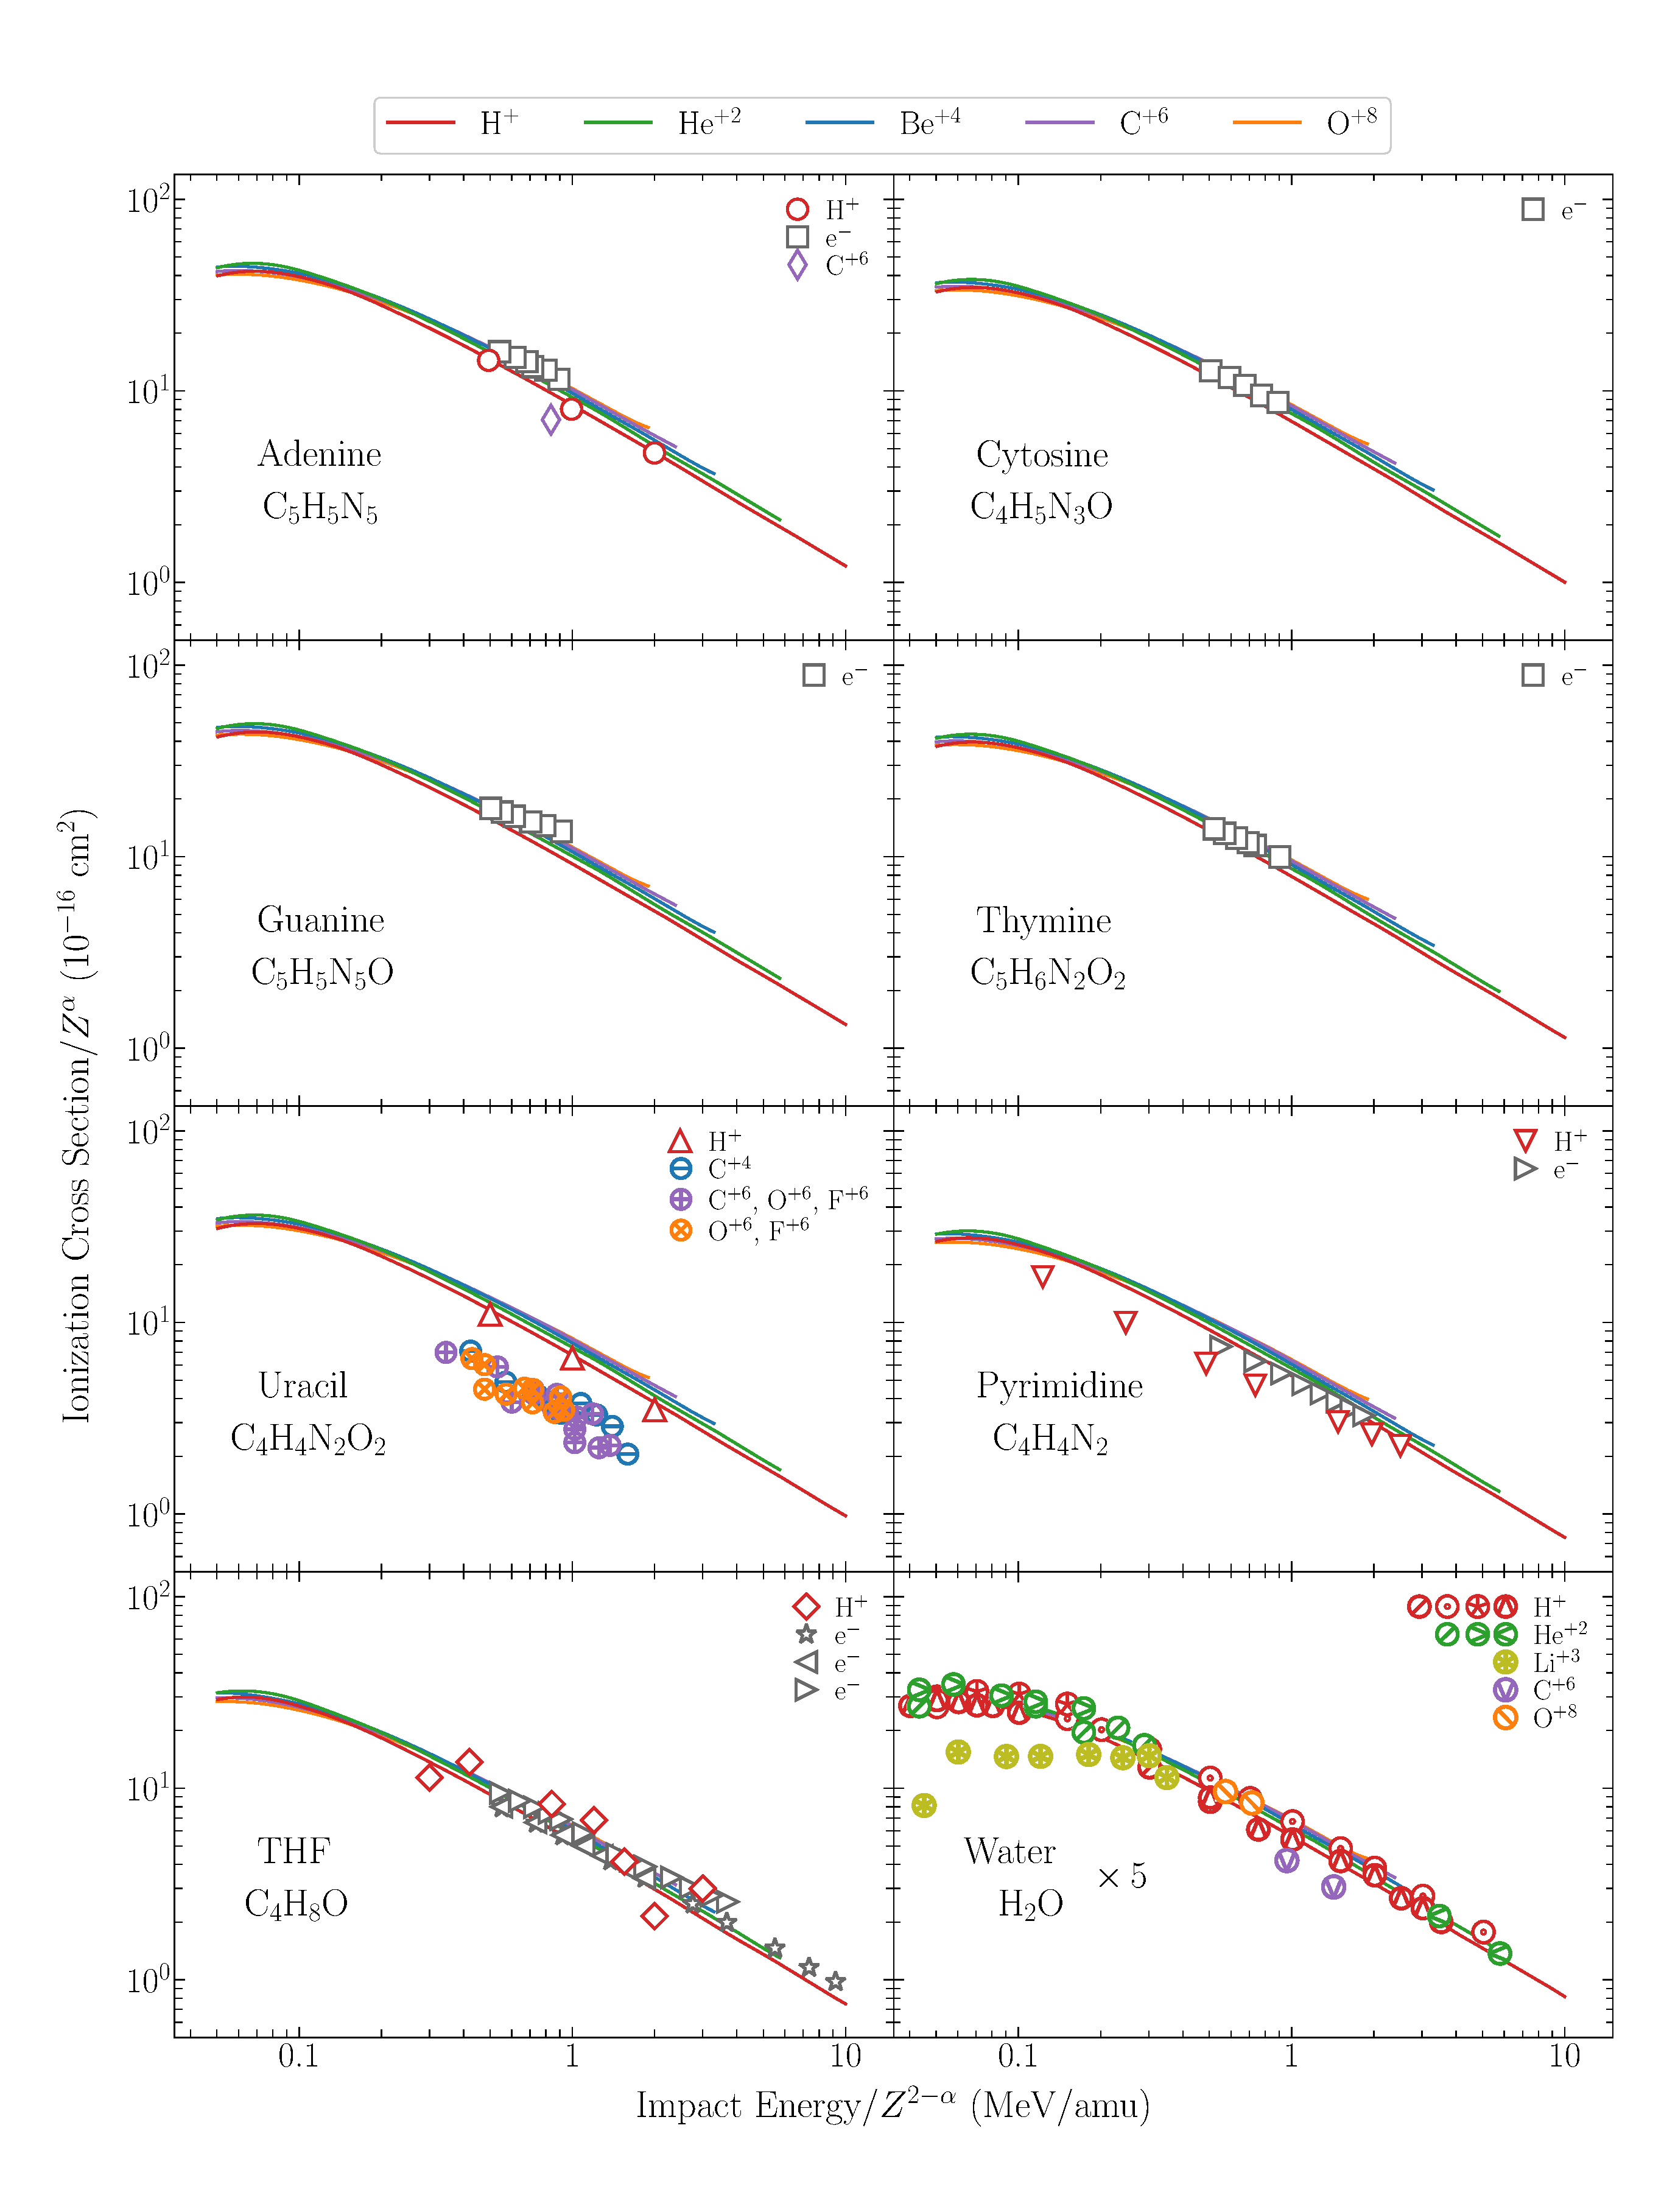
\includegraphics[width=0.87\textwidth]{zscale_alpha.eps}
\caption{(Color online) Scaled ionization cross section $\sigma/Z^{\alpha}$ 
as a function of ion impact energy $E/Z^{2-\alpha}$ with $\alpha=1.2$. 
Colors are associated with the incident ion labeled on top of the figure. 
Curves: present CDW-SSM theoretical results. Symbols: experimental 
impact of \mbox{\LARGE$\color{red}\circ$} H$^+$~\cite{iriki2011} and
{\fontsize{11}{20}$\color{Purple}\pmb{\lozenge}$} C$^{+6}$ 
\cite{tribedi2019} on adenine;
H$^+$ on {\fontsize{11}{20}$\color{red}\pmb{\triangle}$} uracil~\cite{itoh2013}, 
{\fontsize{11}{20}$\color{NavyBlue}\pmb{\ominus}$} C$^{+4}$, 
{\fontsize{11}{20}$\color{Purple}\pmb{\oplus}$} C$^{+6}$, O$^{+6}$, F$^{+6}$, and 
{\fontsize{11}{20}$\color{BurntOrange}\pmb{\otimes}$} O$^{+8}$, 
F$^{+8}$ on uracil~\cite{agnihotri2012,agnihotri2013};
H$^+$ on {\fontsize{11}{20}$\color{red}\pmb{\triangledown}$} 
pyrimidine~\cite{wolff2014}, and 
{\fontsize{10}{20}$\color{red}\pmb{\meddiamond}$} THF~\cite{wang2016};
% water
\mbox{\fontsize{11}{20}$\color{red}\pmb{\odot}$}~\cite{Luna2007}, 
{\fontsize{11}{20}\color{red}$\pmb{\logof}$}~\cite{Rudd86}, 
{\fontsize{11}{20}\color{red}$\pmb{\varowedge}$}~\cite{pRudd85}, 
{\fontsize{11}{20}\color{red}$\pmb{\varoslash}$}~\cite{toburen80} H$^+$,
{\fontsize{11}{20}\color{ForestGreen}$\pmb{\varolessthan}$}~\cite{Ohsawa05},
{\fontsize{11}{20}\color{ForestGreen}$\pmb{\varogreaterthan}$}~\cite{Rudd85},
{\fontsize{11}{20}\color{ForestGreen}$\pmb{\varoslash}$}~\cite{toburen80} He$^{+2}$,
{\fontsize{11}{20}\color{Purple}$\pmb{\ovee}$}~C$^{+6}$ \cite{DalCappello2009,Bhattacharjee17}, and 
{\fontsize{11}{20}\color{BurntOrange}$\pmb{\obslash}$}
O$^{+8}$ \cite{Tribedi_O_water} on water.
Markers~$\square$~\cite{rahman2016}, 
$\rhd$~\cite{bug2017}, 
$\lhd$~\cite{wolf2019}, and 
$\medstar$~\cite{fuss2009} correspond to electron impact ionization with 
the equi-velocity conversion.}
\label{fig:zreduced}
\end{figure*} 

We found two types of $Z$-scaling laws in the literature applicable 
to the intermediate impact energy range. The rule suggested by Janev 
and Presnyakov~\cite{janev1980} 
%depends linearly with ion charge $Z$, considering 
considers $\sigma/Z$ versus $E/Z$ to be the \textit{natural} reduced  
form of the ionization cross section $\sigma$ and the incident ion energy $E$. More recently, Montenegro and co-workers~\cite{dubois13,
montenegro_pra13} suggested an alternative scaling by taking into 
account that the cross section is a function of $Z^2/E$ at high 
energies. Their scaling, given by 
\begin{equation}
 \sigma/Z^{\alpha}=f(E/Z^{2-\alpha}),
\label{eq:Montenegro}
\end{equation}
keeps the $Z^2/E$ relationship for any value of the parameter 
$\alpha$. The authors proposed $\alpha=4/3$ for the ionization of He and 
H$_2$ by differently charged ions~\cite{dubois13}. 
 
Following the work of Montenegro and collaborators, we found that the 
parameter that best converges the CDW-SSM cross sections of the forty 
collisional systems over the broadest energy range is $\alpha=1.2$. 
The validity of this particular scaling is evident in 
Fig.~\ref{fig:zreduced}, where --for each target-- the CDW-SSM curves
corresponding to different ions lay one over the other. 
It is worth noting that our theoretical results are valid for impact
energies above the maximum of the cross sections, which corresponds to 
an impact energy range from 50 keV for H$^+$ to 250 keV/amu for 
O$^{+8}$.

We also examined the experimental data available for the forty 
ion-target systems~\cite{itoh2013,iriki2011,wolff2014,wang2016,
tribedi2019,agnihotri2012,agnihotri2013,Luna2007,Rudd86,Rudd85,pRudd85,
toburen80,Ohsawa05,Bhattacharjee17,Luna_Li_water,DalCappello2009,
Tribedi_O_water} with the $Z^\alpha$-scaling rule. For targets with none or little experimental data, we included
electron impact ionization results~\cite{rahman2016,bug2017,wolf2019,
fuss2009} at high velocity with the corresponding equivelocity 
conversion.
As can be noted, 
most of the data in Fig.~\ref{fig:zreduced} confirm the present 
scaling, even for O$^{+8}$ in water~\cite{Tribedi_O_water}. 
Only two data sets are off our predictions: the ionization cross sections of 
uracil by swift C, O, and F ions from 
Refs~\cite{agnihotri2012,agnihotri2013}% are too low  compared with our CDW-SSM results
; and the values 
for Li$^{+3}$ in water from Ref.~\cite{Luna_Li_water} %spread out from the present theoretical curves
for $E<600$~keV/amu. 
In the case of uracil, recent CTMC calculations by Sarkadi~\cite{sarkadi2016} are also above the experimental values by Tribedi group~\cite{agnihotri2012,agnihotri2013}.


\subsection{Scale with the molecular target}

The good results obtained in the scaling with the ion charge 
encouraged us to further investigate a scaling law that could 
predict values for ionization cross sections of any ion in any 
molecule. To this end, we considered the number of active electrons 
in each molecule $n_e$ proposed in Ref.~\cite{MendezJPB20} and combined 
it with the $Z^\alpha$-scaling from Section~\ref{sec:zscaling}.

In our previous work, we noticed that the CDW ionization cross 
sections, $\sigma_A$, of atomic targets H, C, N, and O  scale with the number of
active electrons per atom $\nu_A$, as \mbox{$\sigma_e=\sigma_A/\nu_A$,} 
where $\nu_A$ is $1$ for H and $4$ for C, N, O, i.e.,
\begin{equation}
 \frac{\sigma_{\mathrm{H}}}{1}\sim
 \frac{\sigma_{\mathrm{C}}}{4}\sim
 \frac{\sigma_{\mathrm{N}}}{4}\sim
 \frac{\sigma_{\mathrm{O}}}{4}\,.
\end{equation}
By %considering
means of the SSM, we define the number of active electrons per
molecule as $n_e=\sum_A n_A \nu_A$. The $n_e$ values for the 
molecular targets considered throughtout this work are displayed in 
Table~\ref{nn}. The scaling with the molecular number of active
electrons proved to give excellent results, as shown in Fig.~6 of 
Ref.~\cite{MendezJPB20}.

\subsection{Scale with the ion charge and \\ the molecular target}

By incorporating the $Z^\alpha$ reduction and the scaling with the %molecular 
number  of active electrons% scaling
, we introduce the scaled and reduced
ionization cross section of molecules $\tilde{\sigma}$, which is 
expressed as a function of $E/Z^{2-\alpha}$, and it is given by
\begin{equation}
 \tilde{\sigma}=\frac{\sigma_e}{Z^{\alpha}}=\frac{\sigma_M/n_e}{Z^{\alpha}}\,,
\label{eq:u-scaling}
\end{equation}
where $\sigma_M$ is the ionization cross section for the molecular target, 
$n_e$ is the number of active electrons per molecule displayed in 
Table~\ref{nn} and the parameter is $\alpha=1.2$.
Fig.~\ref{fig:zalpha} shows the %reduced-scaled 
theoretical and 
experimental values of $ \tilde{\sigma}$ (given by Eq.~(\ref{eq:u-scaling})) %data 
for all the systems displayed in Fig.~\ref{fig:zreduced}% obtained using Eq.~(\ref{eq:u-scaling})
. As can be noted, the scaling works very well
and is independent of the ion charge or the complexity of the molecular
target. 
Our theoretical curves lay in a narrow band valid for any charged ion 
(reduced with $Z^\alpha$) in any molecule (scaled with the number of 
active electrons) with a dispersion of about 20\%. If we consider
the experimental data, the uncertainty of our scaling grows to 30\%, 
which is coverd by %shown with 
the gray area in Fig.~\ref{fig:zalpha}.
It is worth noting that we did not include in this figure %Fig.~\ref{fig:zalpha}
the data for uracil from Refs.~\cite{agnihotri2012,agnihotri2013}, 
and for Li$^{+3}$ on water~\cite{Luna_Li_water}. The discussion 
about these experimental values exceeds the present work. 


\begin{figure*}[!htb]%[h]
\centering
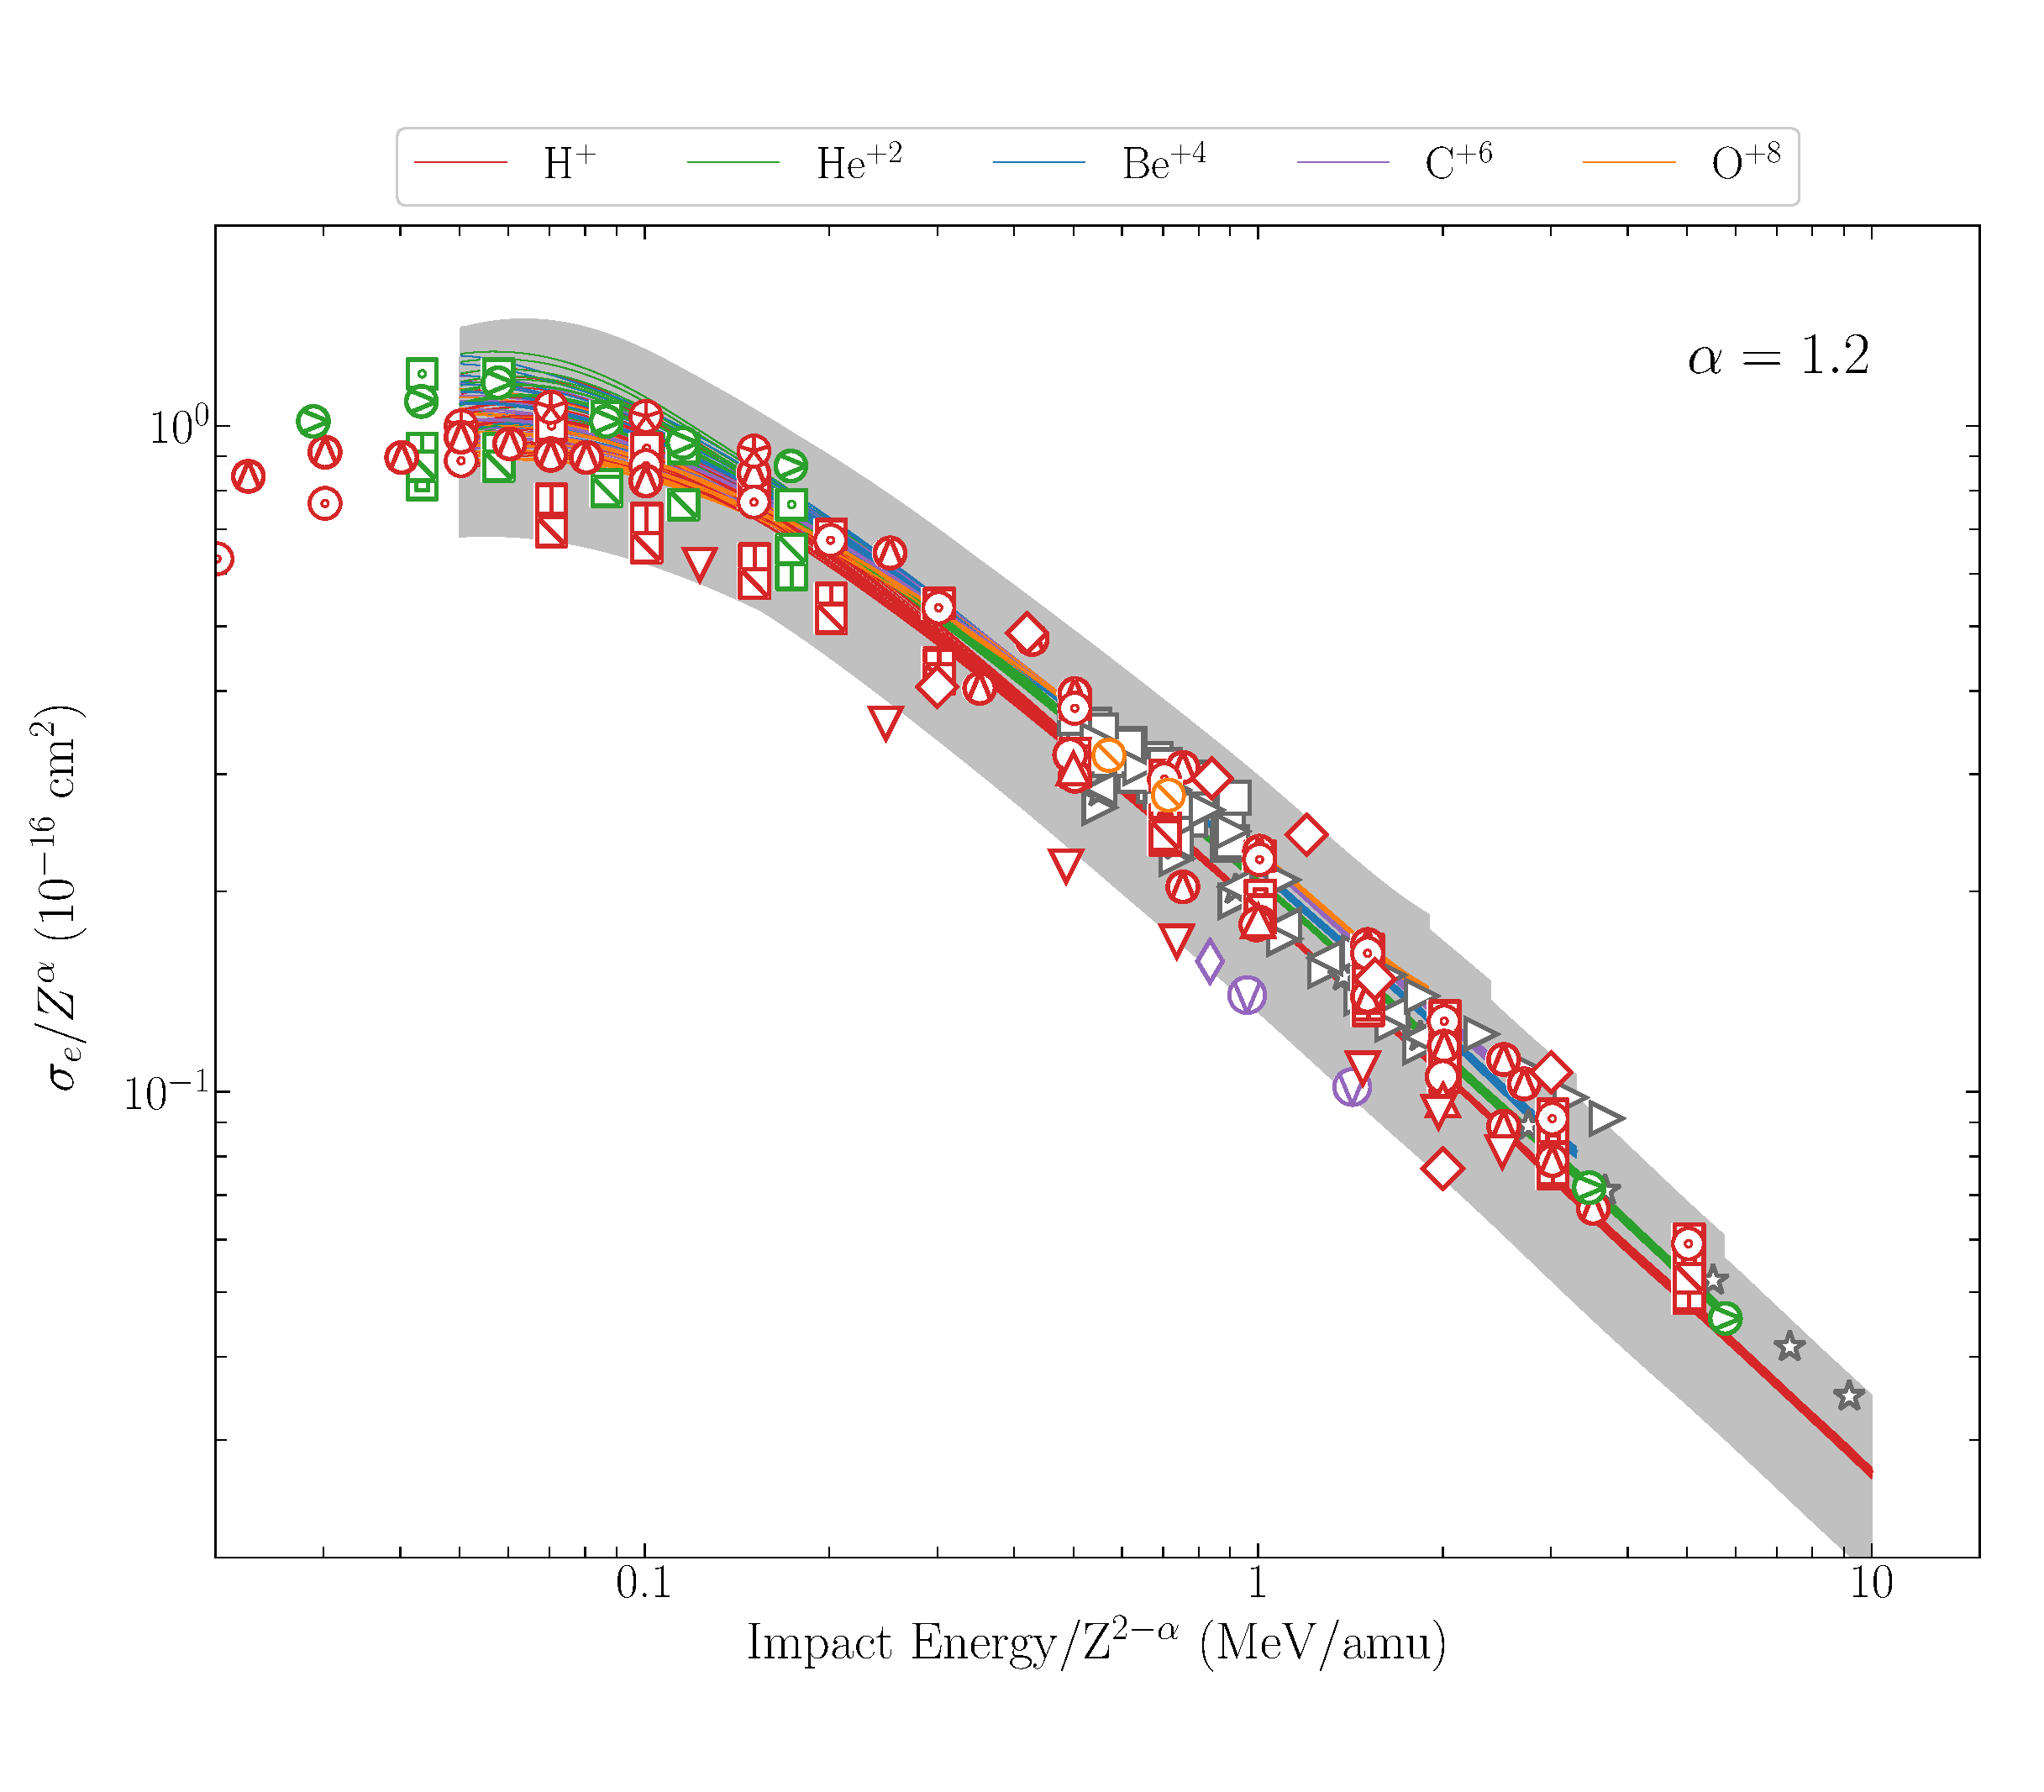
\includegraphics[width=0.75\textwidth]{zmol_werror.eps}
\caption{(Color online) Ionization cross section reduced with the ion
charge $Z$ and scaled with number of active electrons per molecule $n_e$,
given by Eq.~(\ref{eq:u-scaling}) with $\alpha=1.2$. 
Curves: present CDW-SSM theoretical results. 
Symbols: experimental impact of H$^+$ on 
\mbox{\LARGE$\color{red}\circ$} adenine~\cite{iriki2011}, 
{\fontsize{11}{20}$\color{red}\pmb{\triangle}$} uracil~\cite{itoh2013}, 
{\fontsize{11}{20}$\color{red}\pmb{\triangledown}$} pyrimidine~\cite{wolff2014} and 
{\fontsize{10}{20}$\color{red}\pmb{\meddiamond}$} THF~\cite{wang2016};
{\fontsize{11}{20}$\color{Purple}\pmb{\lozenge}$} C$^{+6}$ on adenine \cite{tribedi2019};
\mbox{\fontsize{11}{20}$\color{red}\pmb{\odot}$}~\cite{Luna2007}, 
{\fontsize{11}{20}\color{red}$\pmb{\logof}$}~\cite{Rudd86}, 
{\fontsize{11}{20}\color{red}$\pmb{\varowedge}$}~\cite{pRudd85}, 
{\fontsize{11}{20}\color{red}$\pmb{\varoslash}$}~\cite{toburen80} H$^+$,
{\fontsize{11}{20}\color{ForestGreen}$\pmb{\varolessthan}$}~\cite{Ohsawa05},
{\fontsize{11}{20}\color{ForestGreen}$\pmb{\varogreaterthan}$}~\cite{Rudd85},
{\fontsize{11}{20}\color{ForestGreen}$\pmb{\varoslash}$}~\cite{toburen80} He$^{+2}$,
{\fontsize{11}{20}\color{Purple}$\pmb{\ovee}$}~C$^{+6}$ \cite{DalCappello2009,Bhattacharjee17}, and 
{\fontsize{11}{20}\color{BurntOrange}$\pmb{\obslash}$}
O$^{+8}$ \cite{Tribedi_O_water} on water.
H$^{+}$ impact on 
{\fontsize{11}{20}${\color{red}\pmb{\boxast}}$}~N$_2$, 
{\fontsize{11}{20}${\color{red}\pmb{\boxbox}}$}~O$_2$, 
{\fontsize{11}{20}${\color{red}\pmb{\boxbar}}$}~CO, 
{\fontsize{11}{20}${\color{red}\pmb{\boxbslash}}$}~CO$_2$, and
{\fontsize{11}{20}${\color{red}\pmb{\boxdot}}$}~CH$_4$; 
and He$^{+2}$ impact on 
{\fontsize{11}{20}${\color{ForestGreen}\pmb{\boxast}}$}~N$_2$,
{\fontsize{11}{20}${\color{ForestGreen}\pmb{\boxbox}}$}~O$_2$, 
{\fontsize{11}{20}${\color{ForestGreen}\pmb{\boxbar}}$}~CO, 
{\fontsize{11}{20}${\color{ForestGreen}\pmb{\boxbslash}}$}~CO$_2$, and
{\fontsize{11}{20}${\color{ForestGreen}\pmb{\boxdot}}$} 
CH$_4$~\cite{Rudd85,Rudd1983}, 
{\fontsize{11}{20}${\color{red}\pmb{\varowedge}}$}~H$^{+}$ on 
CH$_4$~\cite{Luna2019}; 
and electron impact on $\rhd$~pyrimidine~\cite{bug2017}, and $\lhd$, 
$\medstar$~\cite{wolf2019,fuss2009} THF.}
\label{fig:zalpha}
\end{figure*} 

We consider this scaling robust enough to be valid for different 
ion--molecule combinations. We tested the generality of our model 
by including in Fig.~\ref{fig:zalpha} several data sets of 
molecular targets not considered previously, such as the measurements 
by Rudd~\textit{et al.}~\cite{Rudd85,Rudd1983} for H$^{+}$ and He$^{+2}$ 
in N$_2$, O$_2$, CH$_4$, CO and CO$_2$, and the recent values by 
Luna~\textit{et al.} \cite{Luna2019} for H$^{+}$ in CH$_4$. 

The good agreement shown in Fig.~\ref{fig:zalpha} summaries the main 
result of this work, and holds the validity of the present scaling for different ions and targets.
%with the ion charge and the number of active electrons in the target. 
Although the theoretical CDW-SSM results are valid for energies above 
the maximum of the cross sections, %it is worth noting from Fig.~\ref{fig:zalpha} that 
the scaling of the experimental data extends 
even to lower impact energies, as can be noted in Fig.~\ref{fig:zalpha}. 
New measurements for other ions and molecules are expected to 
reinforce the present proposal. 

\begin{table}[t]
\begin{center}
\begin{tabular}{|ll|ll|ll|}
\hline
 Molecule & $n_e$ & Molecule          & $n_e$ & Molecule          & $n_e$ \\
\hline
 H$_2$O   & 6  & CO$_2$               & 12 & C$_4$H$_5$N$_3$O     & 37   \\ 
 N$_2$    & 8  & C$_4$H$_8$O          & 28 & C$_5$H$_6$N$_2$O$_2$ & 42   \\ 
 O$_2$    & 8  & C$_4$H$_4$N$_2$      & 28 & C$_5$H$_5$N$_5$      & 45   \\ 
 CH$_4$   & 8  & C$_4$H$_4$N$_2$O$_2$ & 36 & C$_5$H$_5$N$_5$O     & 49   \\ 
 \hline
\end{tabular}
\caption{Number of active electrons per target at intermediate to high 
energies obtained from the CDW calculations~\cite{MendezJPB20}.}
\label{nn}
\end{center}
\vspace{-0.75cm}
\end{table}

%%%%%%%%%%%%%%%%%%%%%%%%%%%%%%%%%%%%%%%%%%%%%%%%%%%%%%%%%%%%%%%%%%%%%%%%
\section{Conclusions}

We present scaling rules for the ionization
cross sections of highly charged ions in biological targets. The first
scaling reduces the nature of the projectile by scaling the cross 
section with the ion charge, $Z^{\alpha}$, as a function of the 
reduced impact energy $E/Z^{2-\alpha}$, with $\alpha=1.2$. The second
scaling considers the molecular characteristic of the target by taking 
into account the number of active electrons per molecule, $n_e$. 
The last scaling law combines the $Z^{\alpha}$-reduction with the
$n_e$-scaling 
of cross section, and it becomes independent of the ion charge and 
the molecular target. The scalings are obtained by means of 
CDW-SSM calculations for five different charged ions in eight targets 
and tested with the available experimental data. The generality of our
independent scaling is proved to be valid in a wide energy range 
by considering a significant number of experimental data sets for 
other collisional systems.

%%%%%%%%%%%%%%%%%%%%%%%%%%%%%%%%%%%%%%%%%%%%%%%%%%%%%%%%%%%%%%%%%%%%%%%%
\section{Acknowlegments}

This work was finantially supported by Consejo Nacional de
Investigaciones Cient\'ificas y T\'ecnicas (CONICET), Agencia 
Nacional de Promoci\'on Cient\'ifica y Tecnol\'ogica (ANPCyT), 
and Universidad de Buenos Aires (UBA).

\begin{thebibliography}{}

% intro --------------------------------------------------------
\bibitem{PhysMed} 
T. Liamsuwan and H. Nikjoo, 
Phys. Med. Biol. \textbf{58}  641--672 (2013).

\bibitem{Mohamad2017}
O. Mohamad, B. J. Sishc, J. Saha, A. Pompos, A. Rahimi, M. D. Story, 
A. J. Davis, D. N. Kim, 
Cancers \textbf{9}, 66 (2017).

\bibitem{Solov2009}
A. V. Solov'yov, E. Surdutovich, E. Scifoni, I. Mishustin, and 
W. Greiner, 
Phys. Rev. E \textbf{79}, 011909 (2009);
% https://link.aps.org/doi/10.1103/PhysRevE.79.011909

\bibitem{Denifl2011}
Denifl S., Märk T.D., Scheier P. 
% The Role of Secondary Electrons in Radiation Damage. 
% In Radiation Damage in Biomolecular Systems. Biological and Medical Physics, Biomedical Engineering. 
Eds: Garc\'ia G\'omez-Tejedor G., Fuss M. 
Springer, Dordrecht (2012) 

\bibitem{water} 
N. A. Gafur, M.  Sakakibara, S. Sano, K. A. Sera, 
% \textit{Case Study of Heavy Metal Pollution in Water of Bone River by Artisanal Small-Scale Gold Mine Activities in Eastern Part of Gorontalo, Indonesia}, 
Water \textbf{10}, 1507 (2018); doi:10.3390/w10111507.

\bibitem{ferrazdias} 
D. Benedetti, E. Nunes, M. Sarmento, C. Porto, C. E. Iochims dos Santos, 
J. Ferraz Dias, J. da Silva,
% \textit{Genetic damage in soybean workers exposed to pesticides: Evaluation with the comet and buccal micronucleus cytome assays},
Mutation Research/Genetic Toxicology and Environmental Mutagenesis,
Volume 752, 28-33 (2013);
% https://doi.org/10.1016/j.mrgentox.2013.01.001.

\bibitem{vera_prl2013} 
P. de Vera, R. Garcia-Molina,I. Abril, and A. V. Solov’yov, 
Phys. Rev. Lett.  110, 148104 (2013).

% our ---------------------------------------------------------
\bibitem{MendezJPB20}
A. M. P. Mendez, C. C. Montanari, and J. E. Miraglia, 
J. Phys. B: At. Mol. Opt. Phys.  \textbf{53}, 055201 (2020).

% others -----------------------------------------------
\bibitem{Quinto20} 
M. A. Quinto, J. M. Monti, C. A. Tachino, P. F. Weck, O. A. Foj\'on, 
C. Champion, R. D. Rivarola, 
% \textit{The physics of irradiation of biological matter by ion beams}, 
Rad. Phys. Chem. \textbf{167}, 108337 (2020);
% https://doi.org/10.1016/j.radphyschem.2019.05.027.

\bibitem{ludde2019}
H. J. L\"udde,  M. Horbatsch and T. Kirchner, 
J. Phys. B: At. Mol. Opt. Phys. \textbf{52}, 195203 (2019).

\bibitem{ludde2018}
H. J. L\"udde, M. Horbatsch and T. Kirchner, 
Eur. Phys. J. B \textbf{91}, 99 (2018).

\bibitem{ludde2016}
H. J. L\"udde, A. Achenbach, T. Kalkbrenner, H.-C. Jankowiak and T. Kirchner,
Eur. Phys. J. D \textbf{70}, 82 (2016).

\bibitem{Champion2012} 
C. Champion, M. E. Galassi, O. Foj\'{o}n, H. Lekadir, J. Hanssen, 
R. D. Rivarola, P. F. Weck, A. N. Agnihotri, S. Nandi, and L. C. Tribedi. 
J. Phys.: Conf. Ser. \textbf{373}, 012004 (2012).


% Z-scaling------------------------------------------------------
\bibitem{janev1980}
R. K. Janev and L. P. Presnyakov 
J. Phys. B: At. Mol. Opt. Phys.  \textbf{13}, 4233 (1980).

\bibitem{dubois13}
R. D. DuBois, E. C. Montenegro and G. M. Sigaud,
AIP Conference Proceeding \textbf{1525}, 679 (2013).

\bibitem{montenegro_pra13} 
E. C. Montenegro, G. M. Sigaud, and R. D. DuBois, 
Phys. Rev. A \textbf{87} 012706 (2013).

% Experimental data ----------------------------------------------

\bibitem{itoh2013} 
A. Itoh, Y. Iriki, M. Imai, C. Champion, and R. D. Rivarola, 
Phys. Rev. A \textbf{88}, 052711 (2013).

\bibitem{iriki2011}
Y. Iriki, Y. Kikuchi, M. Imai, and A. Itoh
Phys. Rev. A \textbf{84}, 052719 (2011). 

%\bibitem{Tabet2010} J. Tabet, S. Eden, S. Feil, H. Abdoul-Carime, B. Farizon, M. Farizon, S. Ouaskit, and T. D. Mark, Phys. Rev. A \textbf{82}, 022703 (2010).

\bibitem{wolff2014}
W. Wolff, H. Luna, L. Sigaud, A. C. Tavares, and E. C. Montenegro
J. Chem. Phys. \textbf{140}, 064309 (2014).

\bibitem{wang2016}
M. Wang, B. Rudek, D. Bennett, P. de Vera, M. Bug, T. Buhr, W. Y. Baek,
G. Hilgers, H. Rabus, 
Phys. Rev. A \textbf{93}, 052711 (2016).

\bibitem{tribedi2019} 
S. Bhattacharjee, C. Bagdia, M. R. Chowdhury, A. Mandal, J. M. Monti, 
R. D. Rivarola, and L. C. Tribedi, 
Phys. Rev. A \textbf{100}, 012703(2019).

\bibitem{agnihotri2012}
A. N. Agnihotri, S. Kasthurirangan, S. Nandi, A. Kumar, M. E. Galassi, 
R. D. Rivarola, O. Foj\'on, C. Champion, J. Hanssen, H. Lekadir, 
P. F. Weck, and L. C. Tribedi. 
Phys. Rev. A \textbf{85}, 032711 (2012).

\bibitem{agnihotri2013}
A. N. Agnihotri, S. Kasthurirangan, S. Nandi, A. Kumar, C. Champion, 
H. Lekadir, J. Hanssen, P. F. Weck, M. E. Galassi, R. D. Rivarola, 
O. Foj\'on and L. C. Tribedi, 
J. Phys. B: At. Mol. Opt. Phys. \textbf{46}, 185201 (2013).

% H+ in water-------------------------------------
\bibitem{Luna2007}
H. Luna, A. L. F. de Barros, J. A. Wyer, S. W. J. Scully, J. Lecointre, 
P. M. Y. Garcia, G. M. Sigaud, A. C. F. Santos, V. Senthil, M. B. Shah, 
C. J. Latimer, and E. C. Montenegro,
Phys. Rev. A \textbf{75}, 042711 (2007).

\bibitem{Rudd86} 
M. A. Bolorizadeh and M. E. Rudd, 
Phys. Rev. A \textbf{33}, 888 (1986). 

\bibitem{pRudd85} 
M. E. Rudd, T. V. Goffe, R. D. DuBois, L. H. Toburen, 
Phys. Rev. A \textbf{31}, 492 (1985). 

\bibitem{toburen80} 
L. H. Toburen, W. E. Wilson and R. J. Popowich,
Radiat. Res. \textbf{82}, 27--44 (1980).

% He$^{+2}$ in water---------------------
\bibitem{Ohsawa05}
D. Ohsawa, Y. Sato, Y. Okada, V. P. Shevelko, and F. Soga
Phys. Rev. A \textbf{72}, 062710 (2005).

\bibitem{Rudd85} 
M. E. Rudd, T. V. Goffe, and A. Itoh, 
Phys. Rev. A \textbf{32}, 2128 (1985).


% Li$^{+3}$ in water---------------------------
\bibitem{Luna_Li_water} 
H. Luna, W. Wolff, E. C. Montenegro, Andre C. Tavares, H. J. Ludde, 
G. Schenk, M. Horbatsch, and T. Kirchner, 
Phys. Rev. A \textbf{93}, 052705 (2016).  

% C$^{+6}$ in water--------------------------
\bibitem{DalCappello2009}
C. Dal Cappello, C. Champion, O. Boudrioua, H. Lekadir, Y. Sato, 
D. Ohsawa, 
Nuclear Instruments and Methods in Physics Research B 267 (2009) 781--790.

\bibitem{Bhattacharjee17}
S. Bhattacharjee, S. Biswas, J. M. Monti, R. D. Rivarola, and 
L. C. Tribedi,
Phys. Rev A \textbf{96}, 052707 (2017).

%O$^{+8}$ in water -------------------------------
\bibitem{Tribedi_O_water} 
S. Bhattacharjee, S. Biswas, C. Bagdia, M. Roychowdhury, S. Nandi, 
D. Misra, J. M. Monti, C. A. Tachino, R. D. Rivarola, C. Champion and 
L. C. Tribedi, J. 
Phys. B: At. Mol. Opt. Phys. \textbf{49,}  065202 (2016).

% electron impact --------------------------
\bibitem{rahman2016}
M. A. Rahman and E. Krishnakumar,
Electron ionization of DNA bases,
J. Chem. Phys. \textbf{144}, 161102 (2016).


\bibitem{bug2017}
M. U. Bug, W. Y. Baek, H. Rabus, C. Villagrasa, S. Meylan, 
A. B. Rosenfeld,
Rad. Phys. Chem. \textbf{130}, 459--479 (2017).


\bibitem{wolf2019}
W. Wolff, B. Rudek, L. A. da Silva, G. Hilgers, E. C. Montenegro, 
M. G. P. Homem,
J. Chem. Phys. \textbf{151}, 064304 (2019).

\bibitem{fuss2009}
M. Fuss, A. Muñoz, J. C. Oller, F. Blanco, D. Almeida, P. Limão-Vieira, 
T. P. D. Do, M. J. Brunger, G. Garc\'{i}a,
Phys. Rev. A \textbf{80}, 052709 (2009).

\bibitem{sarkadi2016} L. Sarkadi, J. Phys. B: At. Mol. Opt. Phys. \textbf{49} 185203 (2016).


% H+ in CH4 and CO2-----------------------------------------
\bibitem{Rudd1983} 
M. E. Rudd, R. D. DuBois, L. H. Toburen, and C. A. Ratcliffe, 
T. V. Goffe, 
Phys. Rev. A \textbf{28}, 3244 (1983).

\bibitem{Luna2019} 
H. Luna, W. Wolff, and E. C. Montenegro, L. Sigaud, 
Phys. Rev. A \textbf{99}, 012709 (2019).

%%%%%%%%%%%%%%%%%%%%%%%%%%%%%%, %%%%%%%%%%%%%%%%%%%%%%%%%%%%%%%%%%%%%%%%%%%%%%%%

\end{thebibliography}

\end{document}

